%%%%%%%%%%%%%%%%%%%%%%%%%%%%%%%%%%%%%%%%%%%%%%%%%%%%%%%%%%%%%%%%%%% 
%                                                                 %
%                            CHAPTER                              %
%                                                                 %
%%%%%%%%%%%%%%%%%%%%%%%%%%%%%%%%%%%%%%%%%%%%%%%%%%%%%%%%%%%%%%%%%%% 

\chapter{Literature Review}
In this chapter, we will go over the state of the art in the field of object counting. We will go over the techniques commonly used for counting and go in more depth about the topic of few-shot object detection and why it should be applied to our problem. Finally, we will discuss the metrics used to evaluate the performance of the models.

\section{(Crowd) Counting}
Counting networks are quite an established concept in machine learning as numerous papers tackle the issue of counting humans, cars, animals or cells. What those have in common is that they only encompass a small set of possible categories to count and that, as they have a large real-life use, large annotated datasets exist for these problems like ShanghaiTech and COWC. The problem we are trying to solve is a bit different as we want to count a large set of objects and we don't have a large dataset to train on.

The methodology behind heuristic counting networks has three big streams\cite{s22145286}. The first applies a detection method to the image and then counts the number of detected objects. Many different detection methods can be used, from looking for characteristic features to matching the shape of the objects. The second takes a more global approach by first extracting features, textures, gradients and other information from the image as a whole and then using those to count the objects. The third method is not used on static images, but on video. It assumes that the objects are moving in clusters and uses that to predict the movement of the objects and improve detection.

Out of those three methods, the third one is not applicable to our problem as we are trying to detect unmoving objects in a still image.
Both the first and second methods are applicable to our problem, however, both have the problem of requiring a large dataset to train on. We will have to use a method that doesn't require a large dataset to train on, which is where few-shot learning comes in. In the domain of few-shot learning the first method, object detection, is the most common. In the next section, we will go more in-depth about few-shot object detection. %FUTURE WORK: try the second method.

%https://www.mdpi.com/1424-8220/22/14/5286

%https://openaccess.thecvf.com/content/CVPR2022W/L3D-IVU/papers/Ranjan_Vicinal_Counting_Networks_CVPRW_2022_paper.pdf

\section{Few-shot object detection}
%https://arxiv.org/abs/2112.11699
%https://ieeexplore-ieee-org.kuleuven.e-bronnen.be/stamp/stamp.jsp?tp=&arnumber=1597116
%add a reference to the first paper that did it
Few-shot object detection is a technique that has been gaining popularity in the last few years. It allows you to train a model on a small dataset, which is useful in scenarios where it isn't possible to get a large dataset to train due to the cost or the time it would take to get it. Interest in making a model to classify text without a big annotated dataset appeared as early as 2008 with zero-shot learning in \citet{aaai08-132}. The method we will be using, few-shot, differs from zero-shot as we have a few images to train on. The idea behind few-shot is as follows if a human can recognize an object after seeing it a few times, then a machine should be able to do the same. Humans achieve this because they have seen many types of objects and can use that knowledge to extract significant features of a new object\cite{biederman1987recognition}. In essence, few-shot learning does the same. It relies on a large dataset of (similar) objects and then applies the knowledge gained from that to a new object, with fewer examples.

Practically this can be done in two different ways. The first way is taking a pre-trained model and using transfer learning to finetune it on the new small dataset. The second way is meta-learning, where the model learns to learn. This means that the model will learn how it should learn to recognize new objects from a large dataset to then apply that to the small dataset. Both of these methods have their characteristics, which we will go over in the next section.

\subsection{Transfer learning}
Transfer learning is a technique that has been used for a long time in machine learning. In few-shot it allows us to use a model that has been trained on a large dataset as a base and, with a few changes to mitigate the small size of the novel dataset, finetune it on a novel dataset. A prevalent base model is Faster R-CNN\cite{fasterrcnn}, which improves on Fast R-CNN\cite{fastrcnn} by introducing attention mechanisms in the form of a Region Proposal Network (RPN) to provide guidance.

Using transfer learning for few shot object detecting has multiple areas that can and have been improved to increase performance. The largest area is the RPN missing the novel object classes \cite{DBLP:journals/corr/abs-2011-10142, VU2022104398, DBLP:journals/corr/abs-2105-09491, DBLP:journals/corr/abs-2103-05950,rs14143255}.
%https://proceedings.mlr.press/v119/wang20j.html
\subsection{Meta-learning}
Meta-learning is a more recent technique in few-shot detection. The idea behind meta-learning is that the model learns how to learn to detect new objects. The are two different meta-learning principles, single-branch and dual-branch meta-learning. As dual branch meta-learning, displayed in figure \ref{fig:2_dualbranchmeta}, is generally more effective, we will focus on that. Many approaches build on top of Faster R-CNN with a ResNet backbone.\cite{few-shot-comprehensive-survey}

Dual branch meta-learning trains using two branches, a query branch and a support branch. The query branch contains full-size images, while the support set contains cropped images of a single labeled object. Both branches try to extract relevant features from their respective images with a shared backbone. The features from the query branch are processed by an RPN and an RoI align resulting in the query RoIs. The features from the support branch are pooled through global average pooling resulting in a support feature vector. Each support feature vector encodes class-specific information which is used to guide the ROI head to recognize objects of the same class. Aggregating the query RoI with the support feature vector results in category-specific RoIs which are then fed into a shared RoI head for bounding box regression and classification. Because the RoI head is shared, it must generalize across all classes. This is what happens during training, during inference the support branch is no longer needed as the support features for the novel classes are computed once.

\begin{figure}[h]
	\centering
	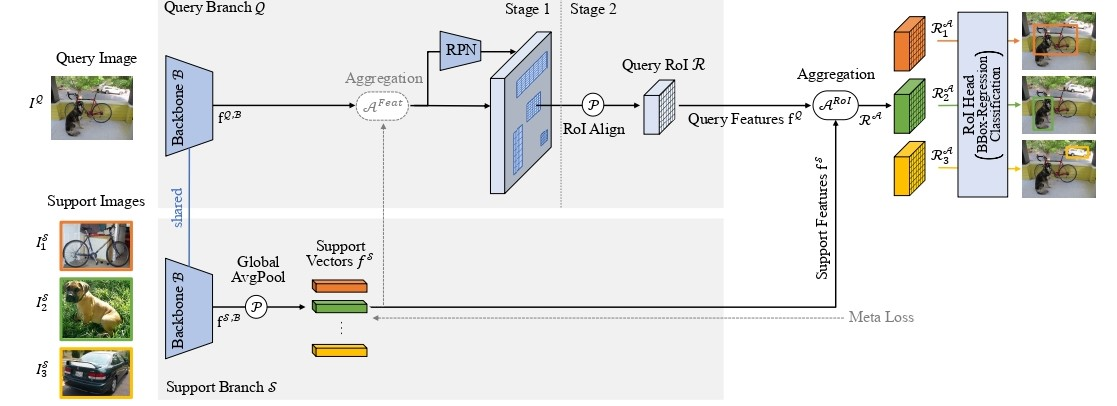
\includegraphics[width=1\textwidth]{2_dualbranchmeta}
	\caption{\label{fig:2_dualbranchmeta} Dual branch meta learning. Image from \citet{few-shot-comprehensive-survey}.}
\end{figure}

\section{Metrics}
In machine learning, it is important to test the model after training, to evaluate its performance. To test the model's accuracy a part of the initial dataset is never used when training. As the unseen inputs are annotated we can find how close the output is to the expected output. With this few key metrics can be calculated. The main metrics we will use are precision, recall and their derivatives. Precision (\ref{eq:precision}) is the ratio of true positives to the total number of positives. Recall (\ref{eq:recall}) is the ratio of true positives to the total number of detectable positives.

\begin{equation}
	Precision = \frac{TruePositives}{True Positives + False Positives}
	\label{eq:precision}
\end{equation}

\begin{equation}
	Recall = \frac{True Positives}{True Positives + False Negatives}
	\label{eq:recall}
\end{equation}

To find if the model output matches the expected output we use the Intersection over Union (IoU) metric. This compares the area of the input and output bounding boxes for each detection by dividing the area of intersection by the area of union. If the IoU, calculated as shown in \ref{eq:IoU}, is above a certain threshold it is considered a detection.

\begin{figure}[h]
	\centering
	\documentclass{standalone}

\usepackage{tikz,pgf}

\begin{document}


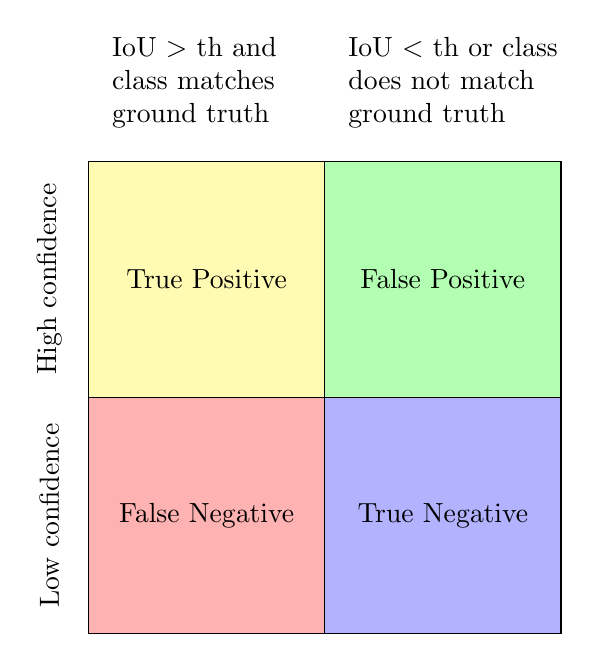
\begin{tikzpicture}
    \draw[draw=black,fill=yellow!30] (0,0) rectangle (3,3);
    \draw[draw=black,fill=green!30] (3,0) rectangle (6,3);
    \draw[draw=black,fill=red!30] (0,-3) rectangle (3,0);
    \draw[draw=black,fill=blue!30] (3,-3) rectangle (6,0);
    
    \node at (1.5,1.5) {True Positive};
    \node at (4.5,1.5) {False Positive};
    \node at (1.5,-1.5) {False Negative};
    \node at (4.5,-1.5) {True Negative};

    \node[text width=2.8cm] at (1.7,4) {IoU \begin{math}>\end{math} th and class matches ground truth};
    \node[text width=2.8cm] at (4.7,4) {IoU \begin{math}<\end{math} th or class does not match ground truth};
    \node[rotate=90] at (-0.5,1.5) {High confidence};
    \node[rotate=90] at (-0.5,-1.5) {Low confidence};
\end{tikzpicture}


\end{document}
	\caption{\label{fig:2_IoU_det} IoU and class match to find the type of detection.}
\end{figure}

\begin{equation}
	\text{IoU} = \frac{\text{area of intersection}}{\text{area of union}}
	\label{eq:IoU}
\end{equation}

Each detection is then evaluated based on how confident the model is and if the detected class matches the ground truth. Below is a list of all the different types of detections:

\begin{itemize}
	\item True positive: The model correctly detects an object and the IoU is above the threshold.
	\item False positive: The model detects an object but the IoU is below the threshold or the model mislabels the object.
	\item False negative: The model does not detect an object but it should have.
	\item True negative: The model does not detect an object and it should not have, this is not used in the metrics as it is not very useful.
\end{itemize}

The threshold between high and low confidence can be varied, a high threshold will result in a low recall but high precision. A low threshold will result in a high recall but low precision. Plotting the precision and recall against the threshold results in a precision-recall curve.

Averaging the precision across all recall levels results in the average precision (AP) metric. Averaging the AP over all classes results in the mean average precision (mAP) metric. The mAP is the most common metric used to evaluate object detection models.

\section{State of the art}
In this section, we will go over the state of the art in few-shot object detection with both transfer learning and meta-learning.
\subsection{Transfer learning}
Transfer learning, as previously discussed, takes a model trained on a large dataset and finetunes it on a novel dataset. In this section, we will go over the state of the art in few-shot object detection with transfer learning.

\subsubsection{A Low-Shot Transfer Detector for Object Detection(\citet{LSTD})}
\citet{LSTD} proposes a new architecture, designed to mitigate transfer learning difficulties in few-shot detection by combining Single Shot Detector (SSD) and Faster R-CNN into Low-Shot Transfer Detector (LSTD). The LSTD architecture is shown in figure \ref{fig:2_LSTD}. In LSTD bounding box regression is first performed according to SSD. The advantage of using SSD is that all classes share a single bounding box regressor, making it suitable for pretraining on a large dataset. The object detection is performed according to a modified Faster R-CNN. Faster R-CNN is modified, replacing the fully connected layers with two convolutional layers, to reduce overfitting.

On the ImageNet2015 dataset, it outperforms Faster R-CNN and SSD. On the VOC2007 and the VOC2010 dataset, it outperforms weakly and semi-supervised object detection methods when the number of training images is above 1. Note that both the weakly and the semi-supervised approaches require the full training set, so LSTD outperforms them with merely 0.4\% training data.

\begin{figure}[h]
	\centering
	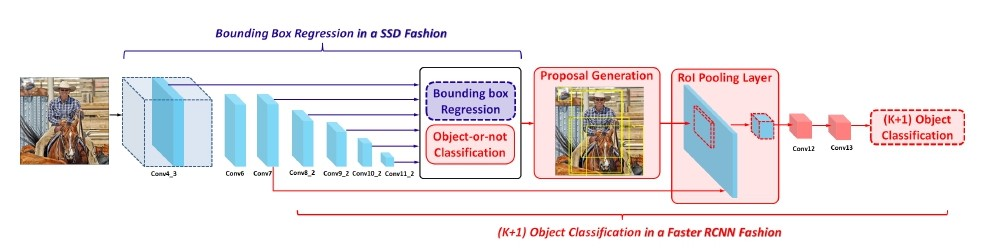
\includegraphics[width=1\textwidth]{2_LSTD_simple.jpg}
	\caption{\label{fig:2_LSTD} LSTD architecture. Image from \citet{LSTD}.}
\end{figure}

\subsubsection{DeFRCN: Decoupled Faster R-CNN for Few-Shot Object Detection (\citet{DeFRCN})}
\citet{DeFRCN} extends Faster R-CNN\cite{fasterrcnn} by introducing Gradient Decoupled Layers (GDL) and Prototypical Calibration Block to create Decoupled Faster R-CNN (DeFRCN). The DeFRCN architecture is shown in figure \ref{fig:2_DeFRCN}.

During forward propagation, the GDLs apply an affine transformation layer to enhance feature representation and perform forward decoupling. During backward propagation, the GDL takes the gradient from the subsequent layer, multiplies it with a constant and passes it to the preceding layer. This reduction ensures that the update speed of the backbone is slower than the update speed of the connected network, this prevents overfitting due to the small dataset. In practice, the gradient between the backbone and the RPN is set to 0 as the RPN is largely class-agnostic, and the gradient between the RPN and the RCNN Head is set to 0.75 during base training and 0.01 during fine-tuning.

The Prototypical Calibration Block (PCB) is a metric-based score refinement module. It aims to eliminate high-scored false positives and remedy low-scored massing samples. It consists of a strong classifier from an ImageNet pre-trained model, an RoI-align layer and a prototype bank. In practice it first extracts the original image feature maps, it then employs RoI-align with ground-truth boxes to produce instance representations. Based on these features the support set is shrunk to a prototype bank. When given an object proposal from the fine-tuned few-shot detector, it first performs RoI-align on the predicted box to generate the object features. It then calculates the cosine similarity between the object features and the prototype bank. In the end, a weighted aggregation between the original score and the cosine similarity is performed. The weight is fixed to 0.5 in practice, resulting in equal weight between the original score and the cosine similarity. As the PCB module is offline and does not require any additional training, it can be easily integrated into any existing object detection framework.

On both COCO and VOC datasets, DeFRCN outperforms the state of the art in all but one combination of novel classes and training images.

\begin{figure}[h]
	\centering
	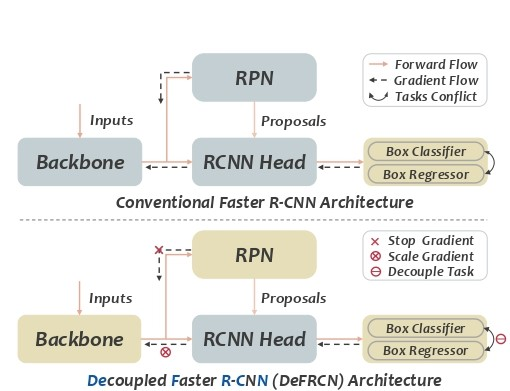
\includegraphics[width=0.5\textwidth]{2_DeFRCN.jpg}
	\caption{\label{fig:2_DeFRCN} DeFRCN architecture. Image from \citet{DeFRCN}.}
\end{figure}

\subsection{Meta-learning}
Meta-learning is a learning paradigm that aims to learn how to learn. It is a form of transfer learning that learns to transfer knowledge from one task to another. In this section, we will go over the state of the art in few-shot object detection with meta-learning.

\subsubsection{Meta R-CNN: Towards General Solver for Instance-level Low-shot Learning (\citet{meta-rcnn})}
\citet{meta-rcnn} proposes a meta-learning approach to few-shot object detection. It extends
Faster /Mask R-CNN\cite{maskrcnn} by introducing a Predictor-head Remodeling Network (PRN). PRN receives few-shot objects drawn from base and novel classes with their bounding boxes or masks, inferring class-attentive vectors corresponding to the classes that few-shot input objects belong to. These class-attentive vectors are then applied to take channel-wise attention on each RoI feature map, after which a binary detection outcome is predicted. The PRN architecture is shown in figure \ref{fig:2_metarcnn}.

\begin{figure}[h]
	\centering
	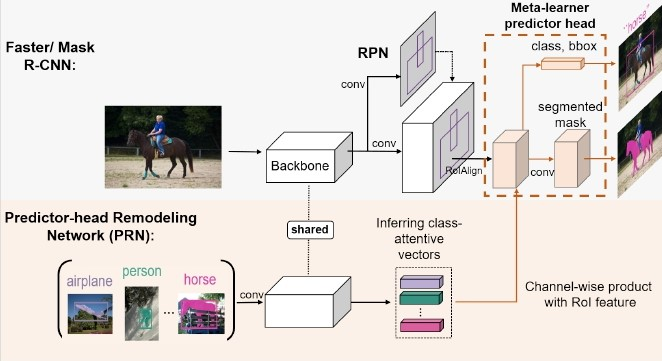
\includegraphics[width=1\textwidth]{2_metarcnn.jpg}
	\caption{\label{fig:2_metarcnn} Meta R-CNN architecture with PRN. Image from \citet{meta-rcnn}.}
\end{figure}

\subsubsection{Meta-DETR: Image-Level Few-Shot Detection with Inter-Class Correlation Exploitation (\citet{MetaDETR})}
\citet{MetaDETR} proposes the first few shot object detector to work on the image level, shown in \ref{fig:2_imagelevelprediction}. It extends Deformable DETR with a Correlational Aggregation Network (CAN) to create Meta-DETR, shown in figure \ref{fig:2_metadetr}. The CAN architecture is shown in figure \ref{fig:2_CAN}. 

\begin{figure}[h]
    \centering
    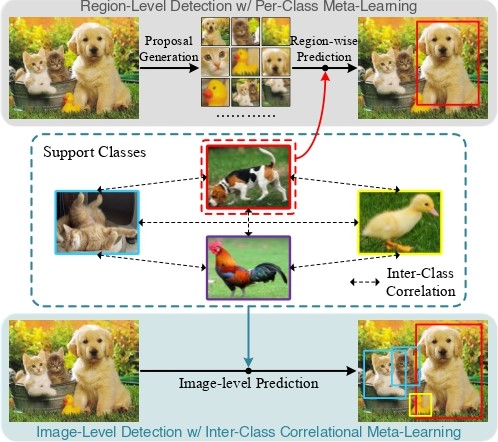
\includegraphics[width=0.4\textwidth]{2_imagelevelprediction.jpg}
    \caption{\label{fig:2_imagelevelprediction} Image level detection. Image from \citet{MetaDETR}.}
\end{figure}

\begin{figure}[h]
    \centering
    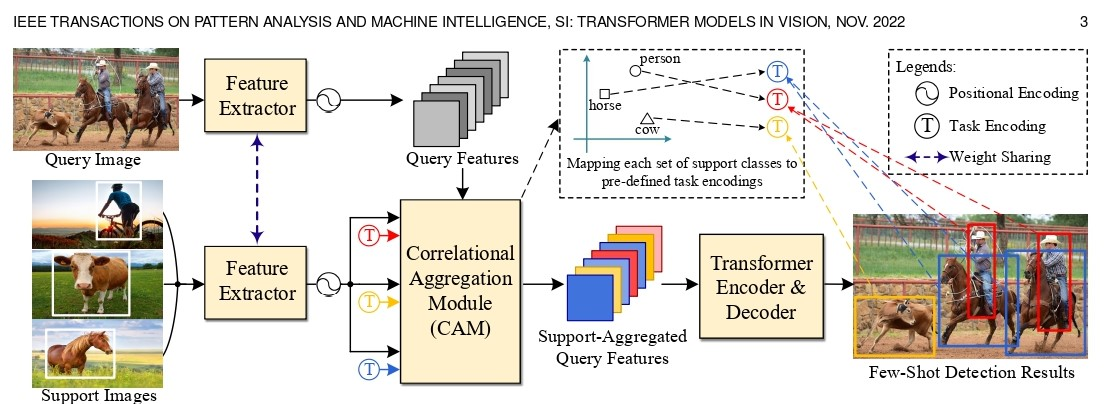
\includegraphics[width=1\textwidth]{2_metadetr.jpg}
    \caption{\label{fig:2_metadetr} Meta-DETR architecture. Image from \citet{MetaDETR}.}
\end{figure}

\begin{figure}[h]
    \centering
    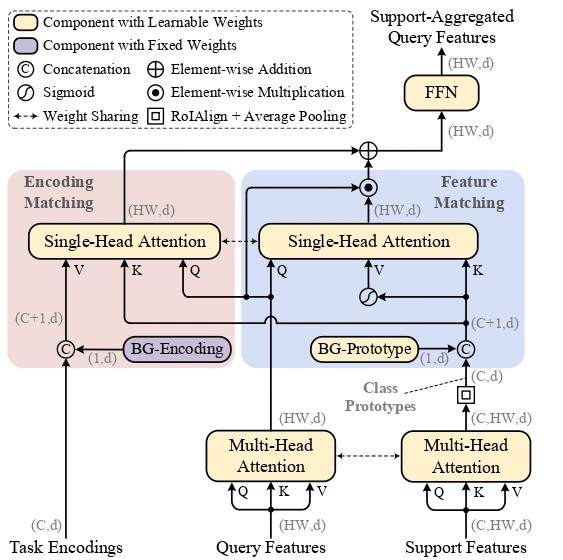
\includegraphics[width=0.4\textwidth]{2_can.jpg}
    \caption{\label{fig:2_CAN} CAN architecture. Image from \citet{MetaDETR}.}
\end{figure}

As shown in fig \ref{fig:2_CAN} the query and support features, extracted by ResNet-101, are first processed by a weight-shared multi-head attention module, encoding them into the same embedding space. Then the prototype for each support class is obtained by applying RoIAlign, followed by average pooling on the support features to get the support prototypes. Feature and encoding matching is then performed on the support prototypes and query features. The sum of the matching scores is then fed to a feed-forward network to obtain the final output.

\section{Conclusion}
In this chapter we have studied object counting, narrowing it down to few-shot object detection to count objects. We then went into more detail about the different ways to implement few-shot learning to detect objects. The sub-field of meta-learning shows the most promise for our problem as it is able to learn the difference between two alike novel classes better than transfer learning.